%%%%%%%%%%%%%%%%%%%%%%%%%%%%%%%%%%%%%%%%%%%%%%%%%%
% Context and objectives
\section{Context, objectives and previous achievements}

\textit{\textbf{Enjeu opérationnel}} : fournir aux agglos des outils d’aide à la décision fiables pour l’élaboration des PCAET, sachant que les émissions qu’elles génèrent représentent environ 2/3 des émissions. Ces outils doivent en particulier répondre à 2 objectifs : permettre aux agglos de contrôler autant que faire se peut leur trajectoire d’émission




%%%%%%%%%%%%%%%%%%%%%%%%
\subsection{Context, objectives and innovative features of the project
}

\notePEPR{Présenter les enjeux scientifiques, les questions de recherche et définir les objectifs du projet et sa pertinence au regard du cadrage général du PEPR.}
\notePEPR{Présenter l’état de l’art national et international en décrivant la pertinence du positionnement scientifique du projet par rapport aux connaissances actuelles. Décrire les principales hypothèses de travail et les principaux choix réalisés.}



\subsection{Main previous achievements}
\notePEPR{Donner les principales réalisations antérieures par les équipes partenaires, démontrer la qualité des résultats déjà acquis soutenant les hypothèses de recherche et les choix réalisés. Ces éléments doivent notamment permettre d’évaluer l’excellence de la recherche et la crédibilité du projet.}

Modelling drivers and instruments:
\begin{itemize}
    \item Modelling low traffic zones in microsimulation \cite{yinEvaluationLowTrafficNeighborhoods2023}
    \item Modelling TOD scenarios \cite{liuTransportLandUse2014, feudoHowBuildAlternative2014}
\end{itemize}

Modelling rupture scenarios:
\begin{itemize}
    \item Implementing rupture scenario in microsimulation approach \cite{kilaniEnvironmentalImpactsBicycling2023}.
\end{itemize}

Modelling the interfaces:
\begin{itemize}
    \item Modelling the interaction between transport and housing markets \cite{kilaniModelEvaluationUrban2023}.
    \item Land-Use and Transport Interaction model implementation \cite{liuTransportLandUse2014, feudoHowBuildAlternative2014}
    \item Modelling transport and health interaction \cite{manoutAssessingRoleDaily2021}

\end{itemize}


\section{Detailed project description}

\subsection{Project outline, scientific strategy}
\notePEPR{Décrire le défi scientifique relevé par le projet.}
\notePEPR{Donner la vision scientifique globale du projet, son caractère original et ambitieux, ainsi que les implications au regard des objectifs du PEPR.}
\notePEPR{Préciser les formes de rassemblement et d’organisation des forces de recherche.}

\subsubsection{First Challenge: Identifying and assessing the contribution of the main drivers for decarbonising territories}

\textbf{Questions à la recherche :} La plupart des outils d’évaluation des gisements, leviers et actions de décarbonation d’un territoire1 actuellement utilisés dans la planification territoriale fonctionnent selon une approche relativement standardisée : on calcule la production d’objectifs opérationnels à réaliser (par exemple : rénover X logements par an), à partir un catalogue d’actions sectorielles et une évaluation d’impacts par ratios statistiques (parfois complétée par des hypothèses issues d’études ou modèles sectoriels). 

Cette approche a le mérite de fournir aux collectivités une vision d’ensemble des leviers de décarbonation sur leur territoire, de « l’effort climatique à viser » et des ordres de grandeur pour l’accélération nécessaire des principales politiques publiques opérationnelles. 

Cependant elle présente de nombreuses limites :
\begin{itemize}
    \item Les évaluations des potentiels et impacts manquent généralement de finesse et de robustesse.
    \item Les évaluations portent sur des objectifs à atteindre. Or, il s’avère difficile de relier l’évaluation des objectifs (approche « macro ») à une véritable évaluation des actions opérationnelles réellement menées ou envisagées. 
    \item Les outils modélisent les gains GES visés, pas les freins ou les impacts non-désirables probables. Or, les nombreux leviers d’action sont ambivalents : les nouvelles technologies peuvent à la fois permettre d’éviter des déplacements et en générer de nouveaux, des incitations économiques peuvent à la fois orienter les comportements vers des pratiques moins coûteuses en énergie et inciter à une surconsommation, par effet rebond.
    \item Plusieurs leviers et freins clés se trouvent soit écartés de l’évaluation, soit abordés marginalement : 
    \begin{itemize}
        \item Les leviers liés à l’organisation spatiale du territoire, à l’usage du sol et aux disponibilités foncières
        \item Les leviers et freins intersectoriels.
        \item Les flux énergétiques et les capacités des systèmes énergétiques, actuels et futurs (y compris nouveaux systèmes innovants)
    \item Les leviers financiers et comportementaux.
    \end{itemize}
\end{itemize}

Les travaux conduits dans \myacronym   devront permettre d’identifier et d’évaluer les principaux leviers d’action, de définir sous quelles conditions ils peuvent être efficaces, de les hiérarchiser en fonction de l’importance de leurs effets sur les émissions et d’améliorer les estimations d’impact chiffrées à différentes échelles. 

Il paraît a priori possible / souhaitable d’agréger les leviers d’action par grandes catégories sectorielles ou plurisectorielles communiquant entre elles (usage du sol, mobilités, bâtiment, systèmes énergétiques), complétés par une réflexion transverse sur des leviers et verrous actuellement difficiles à évaluer dans l’ensemble des secteurs (incitations économiques, nouvelles technologies…).

Urban models describe the spatial and urban configuration of human activities and their interactions. They can express undesired, unsustainable configurations, but can also serve as ideals and targets to guide the action on territories in a strategic, prospective view. As a counter-proposal to the unsustainable urban model of automobile based urban sprawl, Calthorpe formulated the Transit Oriented Development idea \cite{calthorpeNextAmericanMetropolis1993}. More recently, in the same vein, Moreno enunciated the principle of the 15-minute city as an urban model based on proximity \cite{morenoIntroducing15MinuteCity2021}.

We will test urban models as inputs to create scenarios, and we will assess their impact on key parameters of sustainability.  For instance, TOD scenarios will be used to leverage the potential for urban transformations contained in the ambitious (SEM) regional rail projects in French agglomerations.

\textit{\textbf{Enjeux opérationnels }}: être en capacité dans une approche pré-modélisatrice transversale par rapport aux différents secteurs urbains (bâtiment, mobilité, énergie, aménagement / urbanisme) de prendre en considération de manière cohérente les leviers d’action de même importance. Élaborer de cette façon un modèle simplifié qui pourra être ensuite enrichi par sophistication progressive. Associer des indicateurs de suivi aux leviers d’action retenus.

\subsubsection{Second Challenge: Data, in the light of climate change}

\textit{\textbf{Questions à la recherche}}\textbf{ :} Les démarches de planification classiques s’appuient essentiellement sur l’extrapolation de séries statistiques consolidées aux échelles nationale et régionale\footnote{En France, chaque région est dotée d’un Observatoire régional énergie-climat, référence pour les données utilisées dans la planification bas-carbone transverse (Plan climat, schéma directeur des énergies).} , complétée par des données issues de modèles (climatiques, énergétiques et transports notamment) et des données collectées par la collectivité.  

Ces démarches se heurtent aujourd’hui à plusieurs difficultés majeures : 
\begin{itemize}
    \item Une incapacité à alimenter des scénarios de rupture. Le changement climatique introduit des ruptures qui entachent sérieusement la pertinence de l’utilisation de ces séries statistiques, notamment pour ce qui est de leur profondeur temporelle. Sans renoncer complètement à l’utilisation des séries statistiques, il convient de faire appel au moins de manière complémentaire à d’autres méthodes : approches probabilistes, préférences déclarées, IA…). 
    \item L’éparpillement et l’hétérogénéité des sources de données, le manque de finesse des données utilisées pour les exercices de planification à grande échelle (plan climat, documents stratégiques pour la rénovation des logements sur un territoire…) et des donnes parfois très fines issues d’études ou de modèles.
    \item La difficulté de renouveler rapidement et régulièrement la donnée nécessaire à la planification et au pilotage des plans d’action.
\end{itemize}

\textit{\textbf{Enjeux opérationnels :}} être en capacité de formuler et d’évaluer des scénarios de rupture, donner une profondeur temporelle aux méthodes et outils d’aide à la décision qui seront in fine proposés.  

\subsubsection{Third Challenge: Methods and modelling tools}

\textit{\textbf{Questions à la recherche}}: assembler dans une méthode d’évaluation cohérente et intersectorielle l’ensemble des éléments précédemment établis, et réunir ou développer les modèles et données nécessaires à sa réalisation. Il conviendra notamment de préciser les interactions entre secteurs pris en compte. Une approche de type « land use » peut s’avérer pertinente. Elle suppose notamment qu’y soit intégré par rapport aux approches classiques le secteur énergie (non seulement prise en compte des consos d’énergie dans les bâtiments et les transports, mais aussi de la concurrence dans l’occupation des sols entre les EnR\&R et l’aménagement (bâtiments et infrastructures). En outre, les méthodes et outils proposés devront permettre de reconstituer la dynamique des processus générés par les actions conduites (par exemple, une politique en faveur de la diffusion des véhicules électriques va se traduire dans un premier temps par une augmentation des GES du fait de l’énergie grise consommée par la fabrication des batteries avant de produire des effets bénéfiques, dont l’horizon dépend du type de VE produits…).

 \textit{\textbf{Enjeux opérationnels}}\textbf{ : }reconstituer les trajectoires d’émission des territoires pour différents scénarios et plans d’action associés dans une démarche d’aide à la décision.

 
\subsubsection{Fourth challenge: favoriser une recherche scientifique « tirée par l’aval », qui contribue à alimenter les outils d’aide à la décision des collectivités territoriales}

\textbf{Questions à la recherche}: Il y a actuellement une difficulté réciproque pour (1) mobiliser les méthodes et outils issus de la recherche dans le monde opérationnel et (2) alimenter les laboratoires en expression de besoins, cas d’usage concrets et données des collectivités territoriales. L’expérimentation des outils académiques sur un territoire et la mise à disposition des résultats des recherches (open source) ne suffisent pas pour créer cette passerelle indispensable, et mutuellement bénéfique, entre le monde opérationnel et le monde de la recherche. En effet, il existe de nombreux décalages à combler en matière de cas d’usage traités, de présentation des leviers, indicateurs et résultats, ou encore d’écosystème d’outils et données utilisés par les chercheurs et le monde de l’ingénierie territoriale.  

\textbf{Enjeux opérationnels }: À toutes les étapes du projet, croiser les besoins, les méthodes et les outils des collectivités et des chercheurs. Travailler sur les points d’articulation et de passerelles entre des outils et approches de différents niveaux de sophistication. Intégrer les résultats de la recherche dans des outils opérationnels existants ou à développer, notamment la plateforme prévue dans le projet « PLANETE » (LVMT / Efficacity).  

%%%%%%%%%%%%%%%%%%%%%%%%

\subsection{Scientific and technical description of the project}

\notePEPR{Décrire les objectifs scientifiques du projet et la façon dont ces objectifs seront atteints.}
\notePEPR{Présenter les objectifs intermédiaires, les résultats attendus, l’implication des différents partenaires, leurs différentes responsabilités.}
\notePEPR{Préciser les disciplines impliquées dans le projet (selon les disciplines et sous-disciplines HCERES) ainsi que leur rôle dans la réalisation des objectifs.}
\notePEPR{Présenter la cohérence scientifique du projet et de la pluralité scientifique et la crédibilité des jalons proposés, en justifiant les choix méthodologiques, les technologies et éventuellement les infrastructures de recherche utilisées.}
\notePEPR{Décrire les complémentarités des établissements impliqués.}
\notePEPR{Indiquer l’articulation avec d’autres projets, internes ou/et externes au PEPR.}

%%%
\subsubsection{Leviers d'action et interfaces }
\textbf{Leader: \colEFF{J. Laterrasse}}

The bibliography is handled using \textit{BibLaTeX} and \textit{Biber}\footnote{\url{https://en.wikipedia.org/wiki/Biber_(LaTeX)}} instead of \textit{BibTex}, so no problems with diacritics. You do not have to change your \textit{BibTex} file, the syntax is the same.

Let's put a few citations for the example: \cite{kilaniEnvironmentalImpactsBicycling2023,kilaniModelEvaluationUrban2023}. I would recommend putting the URLs directly in the \textit{BibTex} titles, to save space (cf. \texttt{anr\_biblio.bib}).



%%%
\subsubsection{Urban models}
\textbf{Leader: \colUGE{A. L'Hostis}}



%%%
\subsubsection{Data}
\textbf{Leader: \colUGE{O. Bonin}}


%%%
\subsubsection{Models}
\textbf{Leader: \colEFF{M. Wendeln}}


\subsection{Planning, KPI and milestones}
\notePEPR{Présenter l’organisation du travail (tâches, livrables) et son calendrier à l’aide d’un diagramme de Gantt.}
\notePEPR{Identifier les jalons et les livrables avec leur responsable et leur échéance.}
\notePEPR{Donner des indicateurs précis de suivi associés à des cibles éventuelles (KPI).}
\notePEPR{Préciser pour chaque indicateur cible et jalon les risques identifiés et les mesures correctives envisagées.}





We can put some floats here, as examples. A diagram such as the one in Figure~\ref{fig:example}, describing the general organization and the dependencies between the work packages, is likely to appear at some point. A table such as Table~\ref{tab:example} can also be useful, or some equation like eq.(\ref{eq:example}).

\begin{figure}[!ht]
	\centering
	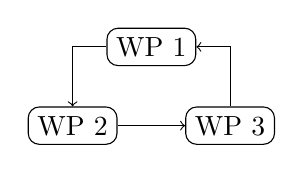
\begin{tikzpicture}
		\draw (0,0) node[draw,rounded corners](WP1) {WP 1};
		\draw (-1, -1) node[draw,rounded corners](WP2) {WP 2};
		\draw (1, -1) node[draw,rounded corners](WP3) {WP 3};
        \draw[->] (WP1) -| (WP2);
        \draw[->] (WP2) -- (WP3);
        \draw[->] (WP3.north) |- (WP1.east);
    \end{tikzpicture}
    \caption{Some diagram representing the relations between the packages.}
    \label{fig:example}
\end{figure}

\lipsum[7]

\begin{table}[!ht]
	\centering
    \begin{tabular}{r r r r}
    	\hline
        \rowcolor{headcolor!20}
    	\textbf{A} & \textbf{B} & \textbf{C} & \textbf{D} \\
    	\hline
        15.99 & 98.98 & 13.67 &  6.25 \\
        16.98 & 65.21 & 63.74 & 25.87 \\
        98.97 &  6.98 & 19.75 & 36.74 \\
        67.39 & 96.84 & 34.14 & 19.85 \\
    	\hline
	\end{tabular}
    \caption{Some example table.}
    \label{tab:example}
\end{table}

\lipsum[8]

\begin{equation}
	y = f(x)
    \label{eq:example}
\end{equation}


%%% WP 0
\wpdef{wp:ProjMgt}{Project Management}
% leader
\textbf{Leaders: \colUGE{A. L'HOSTIS (Univ Eiffel)} \colEFF{M. WENDELN (Efficacity)}}

% description

% Deliverables & co.
\vspace{0.25cm}
\noindent\textbf{Deliverables:} bla bla bla bla.





%%% WP 1
\wpdef{wp:Data}{Drivers for the decarbonation of territories} 
% leader
\textbf{Leader: xxxxxxxxxxxxxx}

% description

\begin{itemize}
    \item état de l’art croisé : approches opérationnelles et scientifiques
    \item hiérarchisation des leviers à « outiller » en priorité (leviers à fort impact GES, où la recherche scientifique a le plus à apporter aux décideurs territoriaux)
    \item \textit{livrable final : }méthode d’évaluation des impacts GES des principaux leviers urbains, s’appuyant sur des outils de modélisation
\end{itemize}


% task
\tdef{tsk:DataST}{some task}


% task
\tdef{tsk:DataOT}{Some other task}


% task
\tdef{tsk:DataLT}{Last task of this WP}


% Deliverables & co.
\vspace{0.25cm}
\noindent\textbf{Deliverables:} some reports.

\noindent\textbf{Success indicators:} scientific publications.

\noindent\textbf{Partners involved:} \colEGS{LMQ}, \colUE{LITA}, \colUT{CGCS}.





%%% WP 2
\wpdef{wp:Classif}{Scenarios}
% leader
\textbf{Leader: xxxxxxxxxxxxxxxxxxx}

% description

\begin{itemize}
    \item Comment concevoir des scénarios de rupture (nécessaires à l’atteinte des objectifs GES des territoires) ? Sur quelles bases ?
    \item Comment les relier aux scénarios opérationnels (utilisés dans la planification et la programmation opérationnelle) ? 
    \item Quels nouveaux outils, modèles et données nécessaires ? 
\end{itemize}

% task
\tdef{tsk:ClassifFT}{First task of this WP}

% task
\tdef{tsk:ClassifAT}{Another task}

% task
\tdef{tsk:ClassifYT}{Yet another task}

% Deliverables & co.
\vspace{0.25cm}
\noindent\textbf{Deliverables:} some reports.

\noindent\textbf{Success indicators:} scientific publications.

\noindent\textbf{Partners involved:} \colINR{LMD}, \colEGS{LMQ}.

%%% WP 3
\wpdef{wp:Exp}{Data?}


\wpdef{wp:Exp}{Implementing models}


\wpdef{wp:Exp}{Other WP?}

Lots 3 à 8 – approfondissements par grandes approches sectorielles : préparation des états de l’art complémentaires, cas d’usage, modèles et données nécessaires

\begin{itemize}
    \item Hypothèses et modèles transverses : hypothèses démographiques et économiques, usage du sol, intégration des données et modèles à différentes échelles spatiales 
    \item Bâtiments et systèmes énergétiques urbains
    \item Transports de personne (tous leviers)
    \item Transports de marchandises (tous leviers)
    \item Référentiel définitif : évaluations carbone, indicateurs complémentaires ; compléments sur les autres secteurs urbains (industrie, déchets, eau…)
\end{itemize}



%%% WP 3
\wpdef{wp:Exp}{Exploiting models results, interaction with territorial stakeholders}
% leader
\textbf{Leader: xxxxxxxxxxxxxxxxxxx}

% description
\begin{itemize}
    \item Une coordination transverse 
    \item Une coordination locale par chaque université sur son territoire d’installation
\end{itemize}

% task
\tdef{tsk:ExpYT}{Yet another task}

% task
\tdef{tsk:ExpTT}{Just two tasks in this WP}

% Deliverables & co.
\vspace{0.25cm}
\noindent\textbf{Deliverables:} some reports.

\noindent\textbf{Success indicators:} scientific publications.

\noindent\textbf{Partners involved:} \colINR{LMD}, \colEGS{LMQ}, \colUE{LITA}, \colTUT{FI}.



\wpdef{wp:Exp}{Valorisation: infusing knowledge, methods, and the practionners toolbox}
% leader
\textbf{Leader: xxxxxxxxxxxxxxxxxxx}
% description
\begin{itemize}
    \item     Production de connaissances scientifiques (publications, colloques, etc.)
    \item Développement des modèles universitaires
    \item Transfert des développements méthodologiques, et des modèles pour enrichir, développer la boîte à outils opérationnels (Efficacity) 
\end{itemize}



%%%
Table~\ref{tab:schedule} shows the list of deliverables of the project, while Figure~\ref{fig:gantt} presents the chronology of the WPs and tasks.

\begin{table}[htb!]
	\centering
	\begin{tabular}{l r l p{8cm} l}
		\hline
        \rowcolor{headcolor!20}
		\textbf{Delivery date} & \textbf{WP} & \textbf{Item} & \textbf{Title} & \textbf{Nature} \\
		\hline
		$t_0$ & \ref{wp:ProjMgt} & WS0 & Project Website & Website \\
		$t_0+3$ & \ref{wp:ProjMgt} & R0.1 & Post-meeting report & Short report \\
		$t_0+9$ & \ref{wp:Data} & W1 & International workshop & Workshop \\
		$t_0+15$ & \ref{wp:ProjMgt} & R0.2 & Post-meeting report & Short report \\
		$t_0+18$ & \ref{wp:Data} & W2 & Great symposium & Workshop \\
		$t_0+21$ & \ref{wp:Data} & R1.1 & Mid-term report on the data & Technical report \\
		$t_0+21$ & \ref{wp:Classif} & R2.1 & Mid-term report on the classification methods & Technical report \\
		$t_0+21$ & \ref{wp:Classif} & R2.2 & Mid-term report on the experiments & Technical report \\
		$t_0+24$ & \ref{wp:ProjMgt} & R0.3 & Post-meeting report & Short report \\
		$t_0+33$ & \ref{wp:Classif} & AP1 & Tool prototype & Software \\
		$t_0+36$ & \ref{wp:Exp} & WS1 & Finalized tool and Webapp & Software \\
		$t_0+36$ & \ref{wp:Exp} & R3.1 & Documentation of the software & Technical report \\
		$t_0+36$ & \ref{wp:Exp} & R3.2 & Final report & Technical report \\
		\hline
	\end{tabular}
	\caption{Task Schedule of the project.}
    \label{tab:schedule}
\end{table}
\noteANR{\textbf{Non-ANR} note: this table does not seem to be required anymore. But it can be useful, let us keep it for now.}

\begin{figure}[!ht]
	\centering
    \begin{ganttchart}[time slot format=isodate-yearmonth, 
		vgrid={dotted,draw=none,draw=none}, %hgrid=true, 
		x unit=0.35cm,									% NOTE: width for a single month
		y unit chart = 0.6cm, bar height=0.6,
		y unit title = 0.5cm, title height=1,
		include title in canvas=false,
        time slot unit=month
	%]{2018-09}{2021-10}
	]{2018-09}{2022-02}
    
	% temporal marks
	\gantttitlecalendar[title/.style={fill=black!30,draw=black}]{year} \\
	\gantttitlecalendar[title/.style={fill=black!20,draw=black}]{month} \\
    
	% horizontal bars
 	\ganttbarbis{WP~\ref{wp:ProjMgt}}{Projet coordination}{2018-10}{2021-07}{blue!50} \\
    
 	\ganttbarbis{WP~\ref{wp:Data}}{Data retrieval}{2018-10}{2020-07}{red!50} \\
 	\ganttbarbis{Task~\ref{tsk:DataST}}{Some task}{2018-10}{2019-02}{red!25} \\
 	\ganttbarbis{Task~\ref{tsk:DataOT}}{Some other task}{2018-10}{2019-08}{red!25} \\
 	\ganttbarbis{Task~\ref{tsk:DataLT}}{Last task of this WP}{2019-03}{2020-07}{red!25} \\
    
 	\ganttbarbis{WP~\ref{wp:Classif}}{Classification methods}{2018-10}{2020-08}{green!50} \\
 	\ganttbarbis{Task~\ref{tsk:ClassifFT}}{First task of this WP}{2018-10}{2020-08}{green!25} \\
 	\ganttbarbis{Task~\ref{tsk:ClassifAT}}{Another task}{2019-03}{2019-10}{green!25} \\
 	\ganttbarbis{Task~\ref{tsk:ClassifYT}}{Yet another task}{2019-11}{2020-07}{green!25} \\
    
 	\ganttbarbis{WP~\ref{wp:Exp}}{Experimental validation}{2019-03}{2021-08}{purple!50} \\
 	\ganttbarbis{Task~\ref{tsk:ExpYT}}{Yet another task}{2019-03}{2020-12}{purple!25} \\
 	\ganttbarbis{Task~\ref{tsk:ExpTT}}{Just two tasks in this WP}{2021-01}{2021-09}{purple!25} \\
    
	% items
 	\ganttmilestone{Items}{2018-10}
 	\ganttmilestone{}{2019-01}
 	\ganttmilestone{}{2019-07}
 	\ganttmilestone{}{2020-01}
 	\ganttmilestone{}{2020-04}
 	\ganttmilestone{}{2020-07}
 	\ganttmilestone{}{2020-10}
	\ganttmilestone{}{2021-07}
 	\ganttmilestone{}{2021-09}
    
	% vertical lines
% 	\drawverticalline{2019-11}{xxxxx}
% 	\drawverticalline{2020-01}{yyyyy}
\end{ganttchart}

	\caption{Gantt Diagram of the project.}
    \label{fig:gantt}
\end{figure}









